%%%%%%%%%%%%%%%%%%%%%%%%%%%%%%%%%%%%%%%%%%%%%%%%%%%%%%%%%%
\section{\label{app:C:FSvsHalfMode}Failure of the free-streaming horizon as measure for non-thermal Dark Matter}
%%%%%%%%%%%%%%%%%%%%%%%%%%%%%%%%%%%%%%%%%%%%%%%%%%%%%%%%%%
\renewcommand{\theequation}{C-\arabic{equation}}
% redefine the command that creates the equation no.
\setcounter{equation}{0}  % reset counter 

Here, we would like to discuss one important point which we had stressed on several occasions throughout the manuscript. Given that we are dealing with highly non-thermal DM spectra, we cannot expect paradigms developed for thermal relics to carry over to this much more general case. In particular, a non-thermal spectrum cannot be described very well by a \emph{single} number, such as a temperature, an average momentum, or a velocity. Given that, we have in fact no reason to believe that a quantity based on an average velocity, such as the free-streaming (FS) horizon $\lambda_{\rm fs}$ as defined in Eq.~\eqref{eq:Def:LambdaFS}, should give us any countable information on the DM spectrum. Yet, it is incorrectly used in many occasions in the literature.

\begin{figure}[ht]
\begin{tabular}{lr}\hspace{-1cm}
 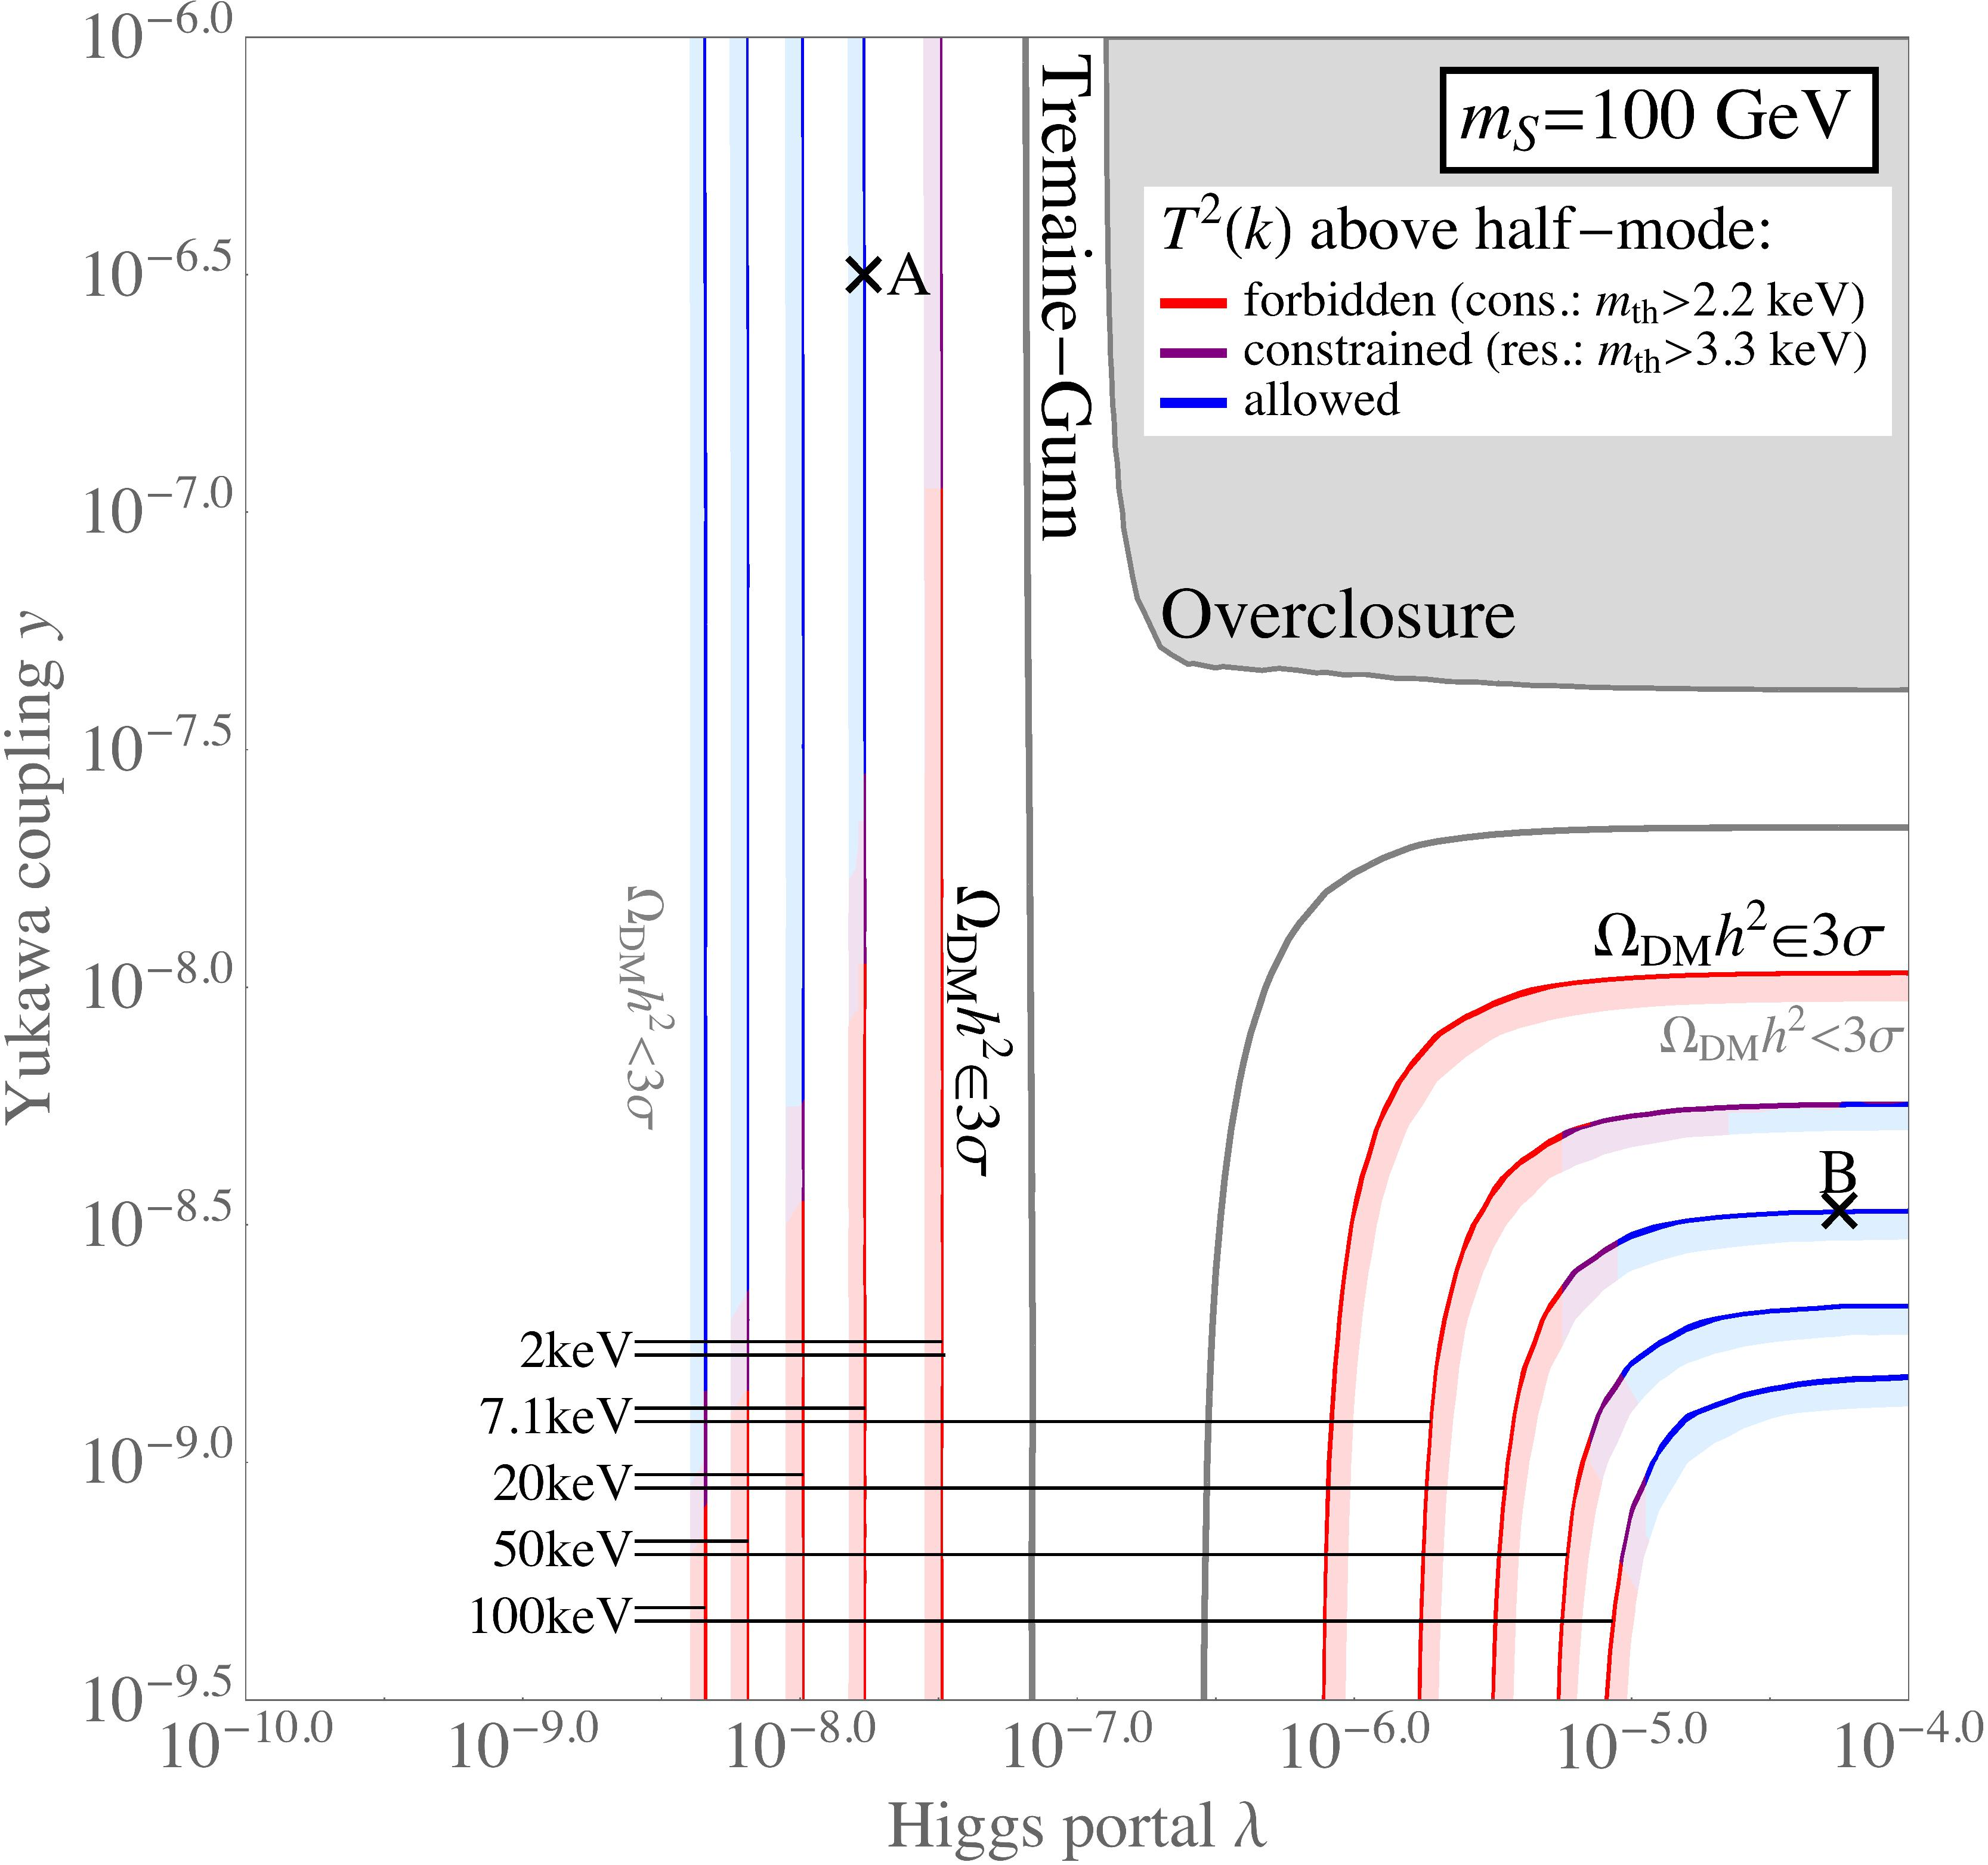
\includegraphics[width=8.3cm]{figures/HM-comparison_100.jpeg} & 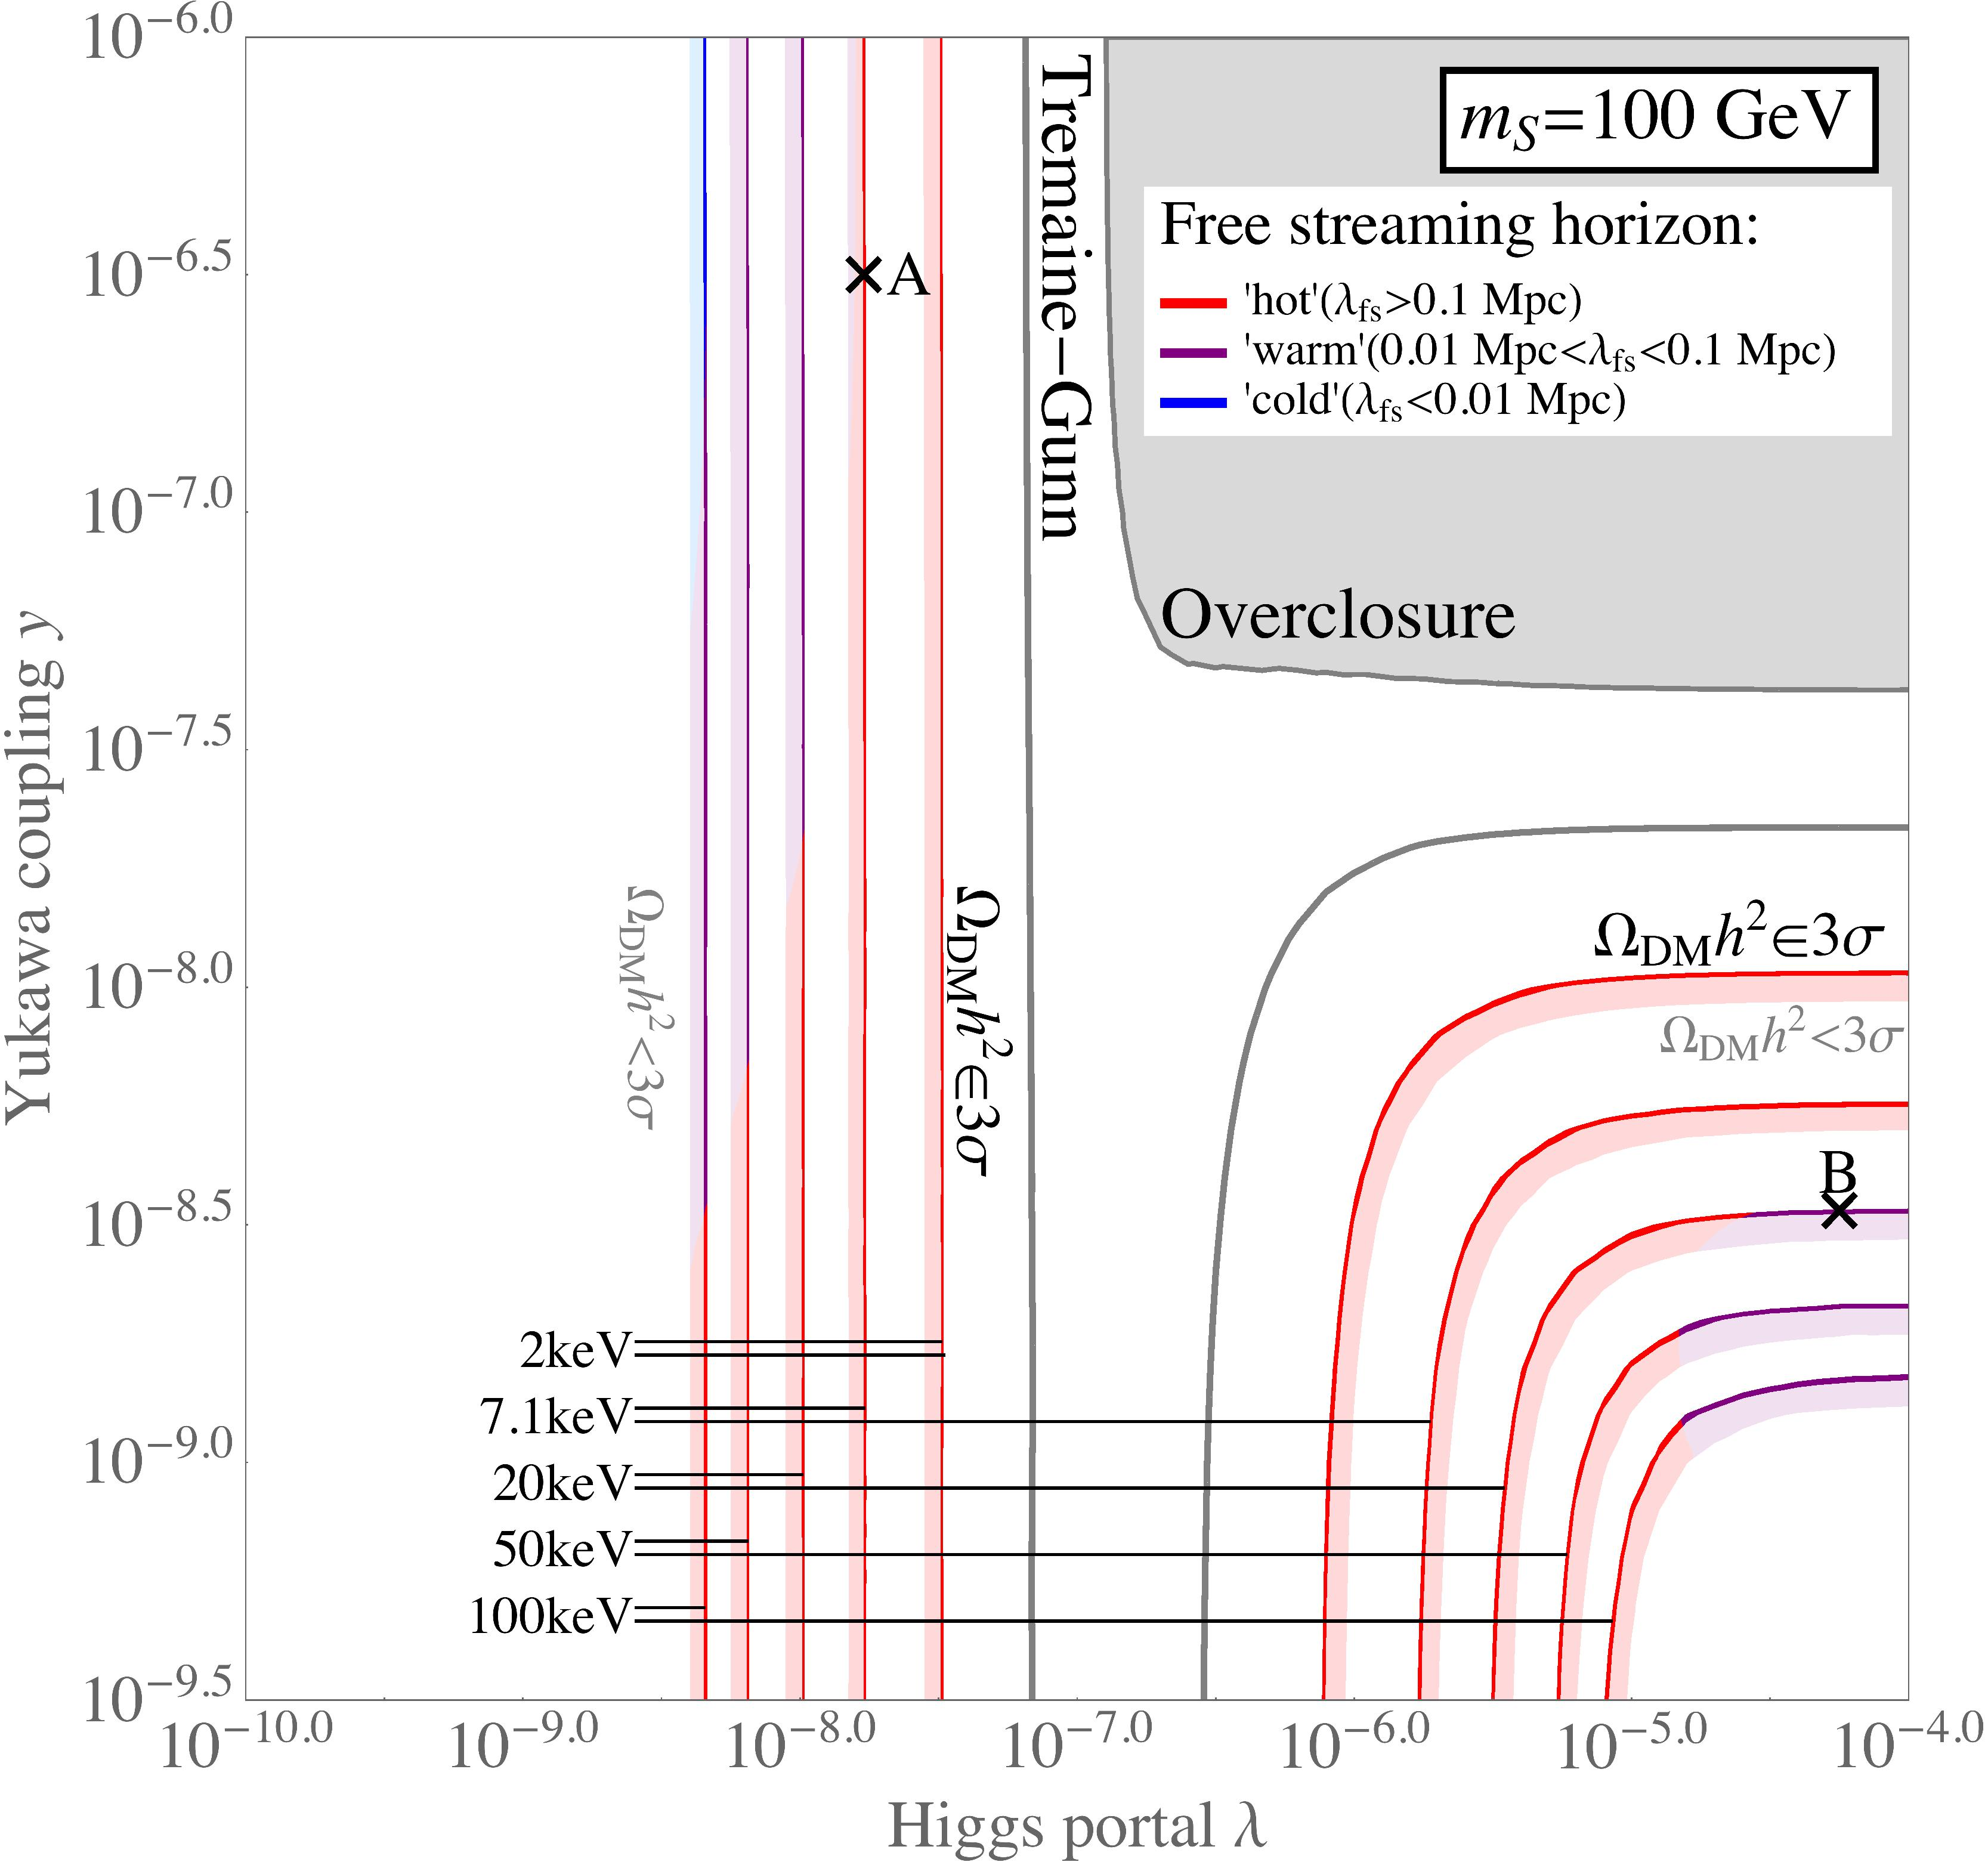
\includegraphics[width=8.3cm]{figures/FS-comparison_100.jpeg}
\end{tabular}
\caption{\label{fig:FS-comparison}Comparison of half-mode analysis (\emph{left}; figure identical to the right Fig.~\ref{fig:small_masses}, except for the model-dependent bounds not being displayed here for simplicity) with the computation of the free-streaming horizon (\emph{right}).}
\end{figure}

In order to clearly illustrate how the FS horizon fails, we compare two versions of an example spaghetti plot, which are depicted in Fig.~\ref{fig:FS-comparison}. Here, on the left panel, we can see the plot for $m_S = 100$~GeV how we obtained it in Sec.~\ref{sec:Results_Light} (this figure is basically identical to the right Fig.~\ref{fig:small_masses}, apart from the missing collider-related bounds which we skipped here in order not to distract the reader). The identical patch of the parameter space is displayed on the right panel of Fig.~\ref{fig:FS-comparison}, however, this time with an analysis based on the FS horizon, classifying the different points as ``cold'', ``warm'', or ``hot'' -- even though, as already explained, these categories do not really suit any non-thermal spectrum. Comparing both plots, one can immedately see that the analysis based on the FS horizon\footnote{This we computed following the numerical computation of the FS horizon as reported in Ref.~\cite{Adulpravitchai:2014xna}, just with a small numerical error in $g_s$ which we have corrected in this version -- the resulting plot would be in between the ``numerical'' and ``analytic'' versions of $\lambda_{\rm fs}$ used in~\cite{Adulpravitchai:2014xna}.} is much more pessimistic than the result based on the half-mode analysis described in Sec.~\ref{sec:Technicalities:Bounds}. While there is no perfect correspondence of the colours red, purple, and blue between the two plots, it is nevertheless evident that some points which are not even constrained by current data in the left plot, seem to be excluded completely when looking at the right plot.

This is particularly true for the two points marked in the plots:
\begin{equation}
 \left\{
 \begin{matrix}
 {\rm A:}\hfill & & m_N = 7.1~{\rm keV},\hfill\hfill\hfill & & \lambda = 10^{-7.77},\hfill\hfill\hfill & & y = 10^{-6.50},\hfill\hfill\hfill\hfill\\
 {\rm B:}\hfill & & m_N = 20~{\rm keV},\hfill\hfill\hfill & & \lambda = 10^{-4.25},\hfill\hfill\hfill & & y = 10^{-8.47}.\hfill\hfill\hfill\hfill
 \end{matrix}
 \right.
 \label{eq:FS-points}
\end{equation}
Obviously, both these points are unconstrained (blue) in the half-mode analysis, while point~A would be classified as ``hot'' (red) in the analyses based on the FS horizon, and even point~B would still be labeled as ``warm'' (purple). This second classification is based on the results obtained for the FS horizon, which turn out to be:
\begin{equation}
 \left\{
 \begin{matrix}
 {\rm A:}\hfill\hfill\hfill & & \lambda_{\rm fs} = 0.117~{\rm MPc} \hfill\hfill\hfill & & \Rightarrow \text{``hot'',}\hfill\hfill\hfill\\
 {\rm B:}\hfill\hfill\hfill & & \lambda_{\rm fs} = 0.089~{\rm MPc} \hfill\hfill\hfill & & \Rightarrow\text{``warm'',}\hfill\hfill\hfill
 \end{matrix}
 \right.
 \label{eq:FS-classification}
\end{equation}
which perfectly matches the classification from the right panel of Fig.~\ref{fig:FS-comparison}.

\begin{figure}[ht]
 \centering
 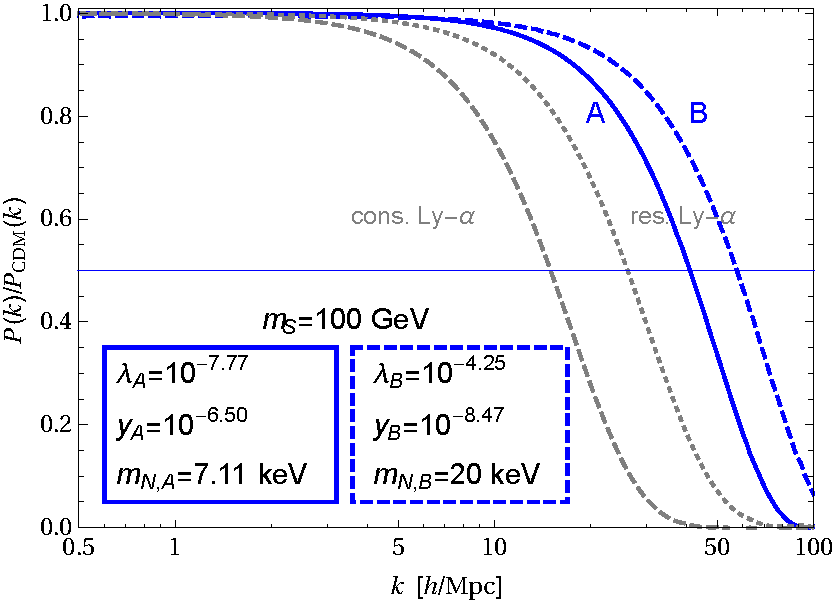
\includegraphics[width=10cm]{figures/Tsquared_mS_100_2SampleCases.pdf}
 \caption{\label{fig:HM-resolution}Squared transfer functions for the points~A and~B marked in Fig.~\ref{fig:FS-comparison}. Even though point~A (point~B) would be completely discarded (strongly constrained) in an analysis based on the FS horizon, both points are in fact in full agreement with data.}
\end{figure}

But how can we be sure that this classification is insufficient? The simplest way is to confront the DM distribution functions with the actual data, which we can do by explicitly displaying the corresponding squared transfer functions in comparison to the Lyman-$\alpha$ data, as done in Fig.~\ref{fig:HM-resolution}. Looking at the curves for both points~A \&~B, we can immediately see that both of them are \emph{not at all} constrained by the data. Thus, both these points are, in fact, even indistinguishable from cold DM, from a structure formation point of view.

Given that this is truly obvious for the two example cases, it serves as a clear example for the FS horizon analysis leading to a conclusion that would be completely incorrect (namely discarding point~A all along, while viewing point~B as borderline case). Thus, as should now be obvious, \emph{the free-streaming horizon is not at all a suitable measure when applied to non-thermal DM distributions}.



